\documentclass{ieee}

\usepackage{graphicx}
\usepackage{amsmath}

\title{DARTS and ProxylessNAS Summaries}
\author{Aamir Jamal, Pawan Shetty, Adam Spindler}

\begin{document}
\maketitle

\section{Introduction}
Neural networks are very complicated systems and require a lot of tuning to work properly on certain tasks such as image classification or text classification. Parameters of the networks are learned by using gradient descent to find a minimum of a loss function that describes the error that the network has on a particular set of training data. The architecture of a network, until recently, has been hand crafted by researchers.


NAS – Neural Network Architecture Search, are algorithmic solutions to automate the manual process of architecture design. Various techniques have been used to find neural network architectures automatically. Reinforcement learning and Evolution has been popular for the task, but is computationally expensive requiring on the order of thousands of GPU hours to find a suitable setup. 

Many techniques for speeding up this process have been proposed, such as restricting the search space to a particular structure or using weights or performance predictions for each developed architecture or sharing weights across multiple architectures. The main cause for such inefficiency is the fact that these Architecture search techniques are considered as black-box optimizations, hence a large number of architectures need to be evaluated to find the most efficient one. 

The two papers examined in this work, DARTS \cite{DARTSMODEL} and ProxylessNAS \cite{cai2018proxylessnas}, propose techniques to create a continuous loss function that includes a representation of the network architecture so that gradient descent can be used to find an optimal architecture in much less time.

Since both the papers are attempting to find the optimal Neural Network Architecture for CNN's (DARTS and Proxyless) and RNN's (DARTS Only). Hence, it would help to briefly overview the functioning of these two varying Neural Networks.


\section{CNN: Convolutional Neural Networks}
\subsection{Overview}
A convolutional neural network (CNN, or ConvNet) is a class of deep neural networks, most commonly used to analyze visual imagery. They typically map an input image tensor to an output classification vector. To do the mapping, multiple hidden layers are used which have varying operations, the typical layer types are :\\
\textbf{- Convolutional Layers} \\
Convolutional Layers are used to emulate the response of an individual neuron to visual stimuli and each convolutional neuron only processes data for its receptive field. They are usually an n $\times$ n matrix that are used as a feature detector or a filter. They act like a window with $n^2$ cells, that slides over every pixel of an image  performing a multiplication on each corresponding pixel value, and then summing the result together to get an output pixel for the next layer. The output is a feature map which is a representation of the image with information that is helpful for the problem that the network is trying to solve.

Although, the feature map will lose a lot of information, the idea of the convolutional filter is to only retain the parts of the image that we are interested in retaining and identifying.
 The brain works in a similar fashion, retaining only certain features and looking at the retained features broadly. Categorizing features broadly is the most practical solution for Image Recognition.
 \begin{figure}[h]
    \begin{center}
    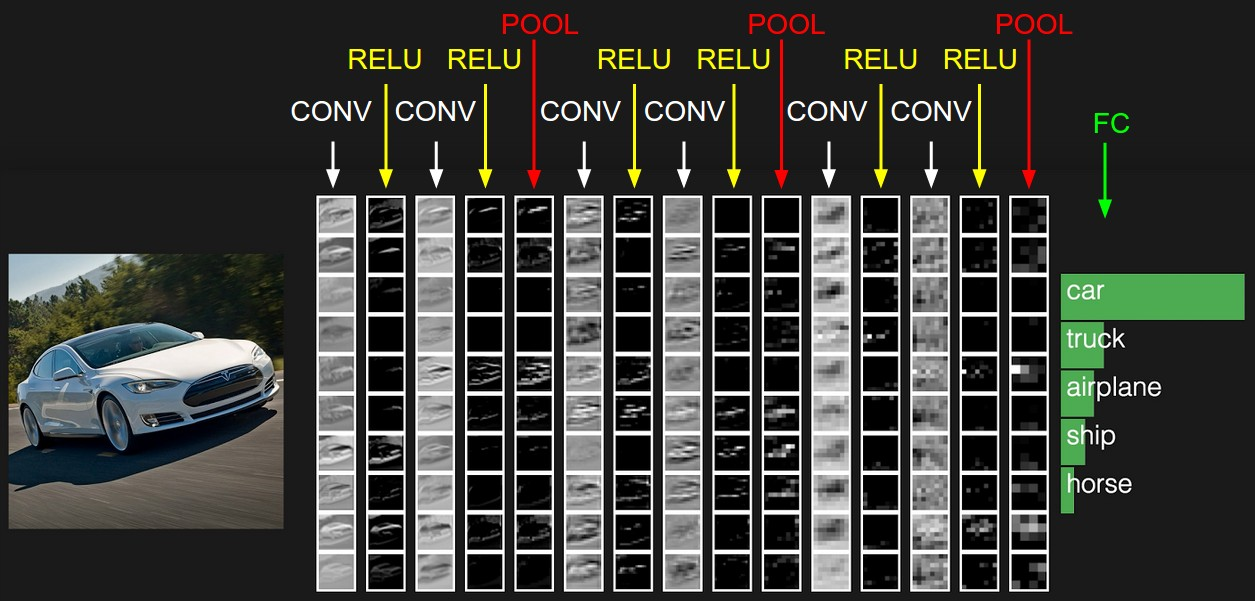
\includegraphics[width=7cm]{images/convnet.jpeg}
    \end{center}
    \label{mbconv_fig}
    \caption{An Example of a Convolutional Neural Net. Each Convolutional Filter helps highlight certain features of an Image. \cite{CONVNETIMAGE}}
\end{figure}

\textbf{- RELU Layers (Activation Functions) }\\
 After each Convolutional layer, there is always a nonlinear layer (or activation layer). Its purpose is to introduce nonlinearity to a system that has been computing linear operations in the previous layers. This is necessary to make sure that the system can learn non-linear functions, and most machine learning models can only be represented as nonlinear functions. Nonlinear functions like tanh and sigmoid were often used in the past, but researchers found out that ReLU layers help the network to train a lot faster without making a significant difference to the accuracy.
 
\textbf{- Pooling Layers} \\
Convolutional networks may include local or global pooling layers. Pooling layers reduce the dimensions of the data by combining output of region in a feature layer together. The combination is done by calculating the average of the previous activations, or computing their max. Reducing the size of the feature map is necessary to eventually arrive at a label vector.

\textbf{- Fully Connected Layers} \\
Fully connected layers connect every neuron in one layer to every neuron in another layer. It is in principle the same as the traditional multi-layer perceptron neural network (MLP). The flattened matrix goes through a fully connected layer to classify the images.

- \textbf{Normalization Layers} \\
There are many types of normalization layers that have been proposed for use in CNN architectures, sometimes with the purpose of implementing inhibition schemes observed in the biological brain. However, these layers have since fallen out of favor because in practice their contribution has been shown to be minimal, if any. 



\section{RNN: Recurrent Neural Networks}
Another field of study where AI has seen a lot of progress in recent years is language modeling for which we use a class of neural networks called recurrent neural network (RNN). We can think of RNNs as multiple copies of the same network, each passing a message to a successor in a sequence. Each element of that sequence performs the same task with the output being dependent on the previous element's computation.  The input to the hidden node in an RNN is both the input from at the current timestep, and the value its own activation in the previous timestep. This can be seen as the RNNs have a memory which captures information about what has been calculated so far.
\begin{figure}[h]
    \begin{center}
    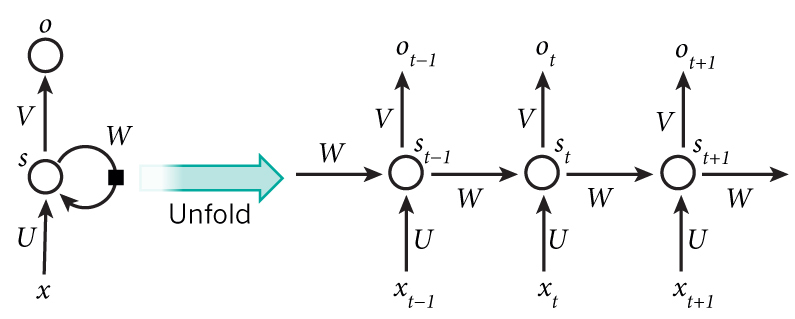
\includegraphics[width=7cm]{images/rnn.jpg}
    \end{center}
    \label{fig:rnn_fig}
    \caption{A recurrent neural network and the unfolding in time of the computation involved in its forward computation. \cite{RNN}}
\end{figure}

In the Fig.2 we can see an RNN being unfolded into a full network. The unfolding of an RNN simply means that we write out the network for its complete sequence. For example, if the sequence we care about is representing a sentence of 6 words, the RNN would be unfolded into a 6-layer neural network, one layer for every input word vector.

\section{Datasets used in the experiments}
The CNN architectures developed in the paper were tested using CIFAR-10 and ImageNet Datasets. Both these Datasets contain a large number of Images, that are used by Researchers and Scientists for testing Visual Recognition.  The RNN architectures were tested using PTB and WikiText-2 Datasets. These are large Tree Banks, that represent both the syntactic and semantic structure of english sentences. They are mainly used in Natural Language Processing Research, to help test the systems developed for speech recognition, etc. A brief understanding of the dataset would help us understand the experiments better.
\subsection{ImageNet}
The ImageNet dataset is a very large dataset containing more than 14 million images that have been hand annotated by crowdsources. Image level annotation indicates whether an object is present or absent in the image. For example, whether a car is present in the image or not. The ImageNet dataset contains more than 20,000 categories and each category consists of several hundred images.
\subsection{CIFAR-10}
Canadian Institute For Advanced Research -10 is one of the most widely used datasets for machine learning researches. There are 10 different classes of images and in each class, there are about 6,000 images of low resolution (32x32). As the images are of low resolution, they can be easily used by researchers to see what works. As this dataset is relatively small, it can be used as a proxy for training a network model.
\subsection{Penn TreeBank (PTB)}
The Penn TreeBank dataset is very commonly used for machine learning of Natural Language Processing. The PTB project annotates naturally occurring text for linguistic structure.
\subsection{WikiText-2}
WikiText-2 is a very large language modeling dataset. It basically is a collection of over 100 million tokens which is extracted from a set of featured Wikipedia articles. When compared, WikiText-2 is over two times larger than the preprocessed version of Penn Treebank dataset. WikiText-2 also preserves punctuations and numbers, which are removed in PTB and also features a much larger vocabulary than PTB.

\section{DARTS: Differentiable Architecture Search}
\subsection{Overview}
The existing architecture search algorithms, that use reinforcement learning (RL) or evolution to discover neural network architectures, are computationally demanding despite their remarkable performance. In these architecture search algorithms, NAS is treated as a black-box optimization problem over a discrete domain, hence a large number of architecture evaluations are required to find the most efficient architecture. Different approaches have been proposed to speed up the search, such as restricting the structure of the search space, weights or performance prediction for each individual architecture and weight sharing/inheritance across multiple architectures, but the techniques still are not scalable. 

 A discrete representation(used in all the past architecture search algorithms) is the most obvious way to encode a network. There are a certain number of hidden layers, each with a specific operation that they perform. The operation types are discrete and so are the number of nodes, so representing it in a continuous way is more difficult. 

DARTS (Differentiable ARchiTecture Search), instead uses a continuous search space, and uses gradient decent on the the Validation Dataset to optimize the Architecture based on a Loss Function. Unlike the techniques used before it, DARTS does not fine-tune specific aspects of the architecture, but instead learns the entire architecture building block.  It is simpler than many existing approaches and can handle both CNNs and RNNs.

\subsection{Search Technique}
DARTS searches for a computation cell as the building block of the final architecture. The learned cell could either be stacked to form a CNN or recursively connected to form an RNN. A cell is a directed acyclic graph with N nodes. A node could be considered as an output of an operation (like a feature map) and the edges can be considered as the operations (like convolution, max pooling, zero, ReLU) themselves. 

Initially the edges are unknown and a combination of all operations are applied on each edge. DARTS uses a joint optimization technique to obtain the mixing probabilities for the architecture and the network weights. It needs to optimize the weights for the architecture that it currently is examining to reduce the training loss on that network. It also needs to optimize the architecture representation to be as good as possible, which is evaluated by taking the validation loss of the network with the current architecture using the weights that it optimized already. 
 \begin{figure}[h]
    \begin{center}
    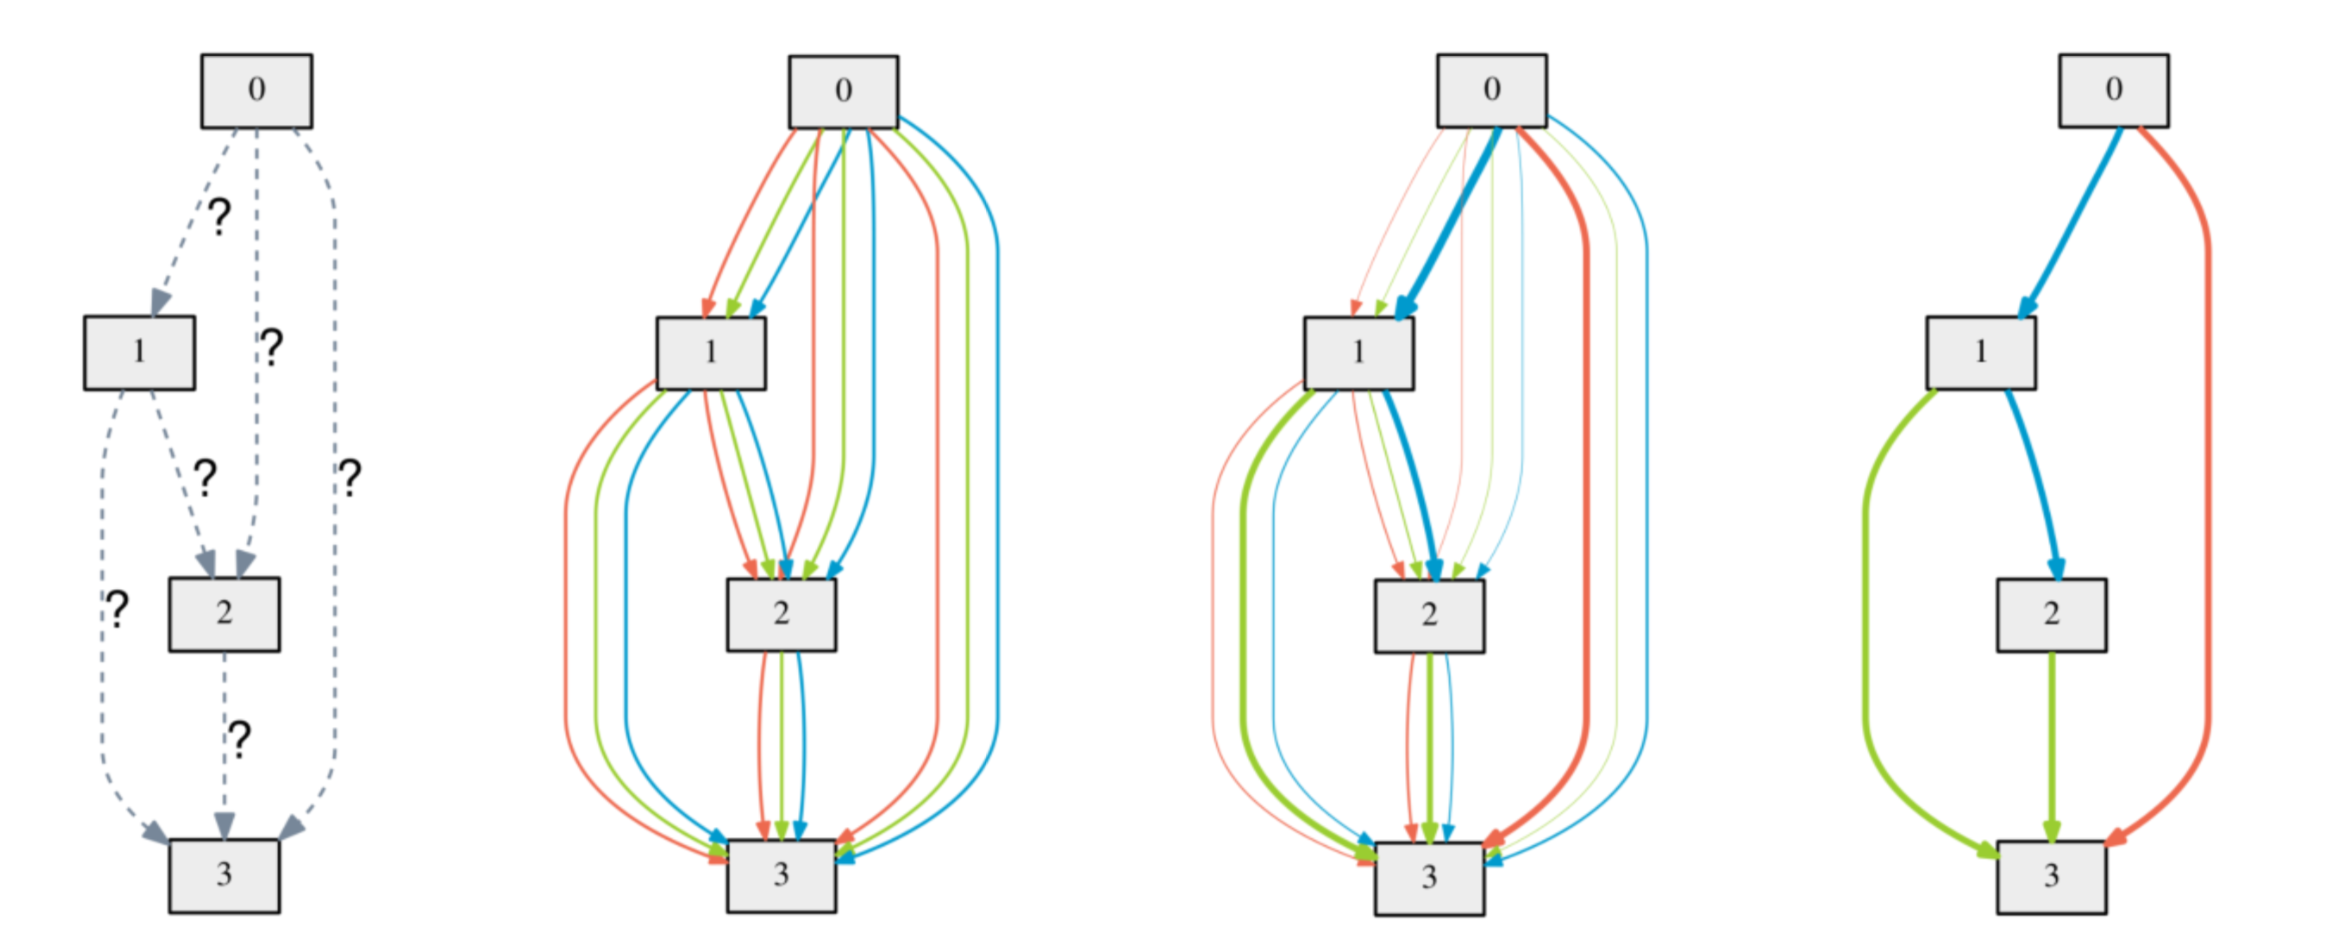
\includegraphics[width=7cm]{images/DARTS.png}
    \end{center}
    \label{mbconv_fig}
    \caption{A cell with four Nodes and various possible operations. \cite{DARTSMODEL}}
\end{figure}

The search begins by computing a softmax over all possible operations that can be performed, reducing the architecture to learning a set of continuous variables. The softmax is used to boost the probability of the operation that has the highest value. A regular max function is non-differentiable, so softmax must be used so that the gradients can be computed. At the end of the search, a discrete architecture is obtained by choosing the most likely operation from the set of all operations. The goal is to jointly learn the architecture $\alpha$ and the weights $w$ within all the mixed operations and using gradient descent to optimize the validation set loss.

Let $L_{train}$ and $L_{val}$ be the training and the validation loss, respectively. The losses are determined by the Architecture $\alpha$ as well as the weights $w$ in the network. The goal of the search is to perform a bilevel optimization on the upper-level variable $\alpha$, Architecture  and the lower-level variable w as follows:\\ \\
$\underset{\alpha}{min}  L_{val}(w^*(\alpha), \alpha)$ \\ 

s.t. $ w^* (\alpha) = argmin_w L_{train}(w, \alpha)$ \\

Calculating the architecture gradient is extremely expensive for each inner optimization, hence a simple approximation technique is proposed to approximate $ w^*( \alpha ) $ by adapting $w$ using only a single training step, without solving the inner optimization. While convergence is not guaranteed, in experiments it is able to reach convergence with a suitable choice of $\xi$ which is the learning rate of training the neural network with the architecture $\alpha$. \\ \\
$\bigtriangledown_\alpha L_{val}(w^*(\alpha), \alpha)$ \\ \\ 
$\approx \bigtriangledown_\alpha L_{val}(w - \xi \bigtriangledown_w L_{train}(w, \alpha), \alpha)$ \\

Each node in the discrete architecture is formed by retaining the top-K strongest operations from the set of all non-zero candidate operations collected from the previous nodes.

\subsection{Experiments}
The experiments consist of two stages, architecture search and architecture evaluation. In the first stage cell architectures are searched for using DARTS, and the best ones are chosen based on their performance on the validation set. In the second stage, the best performing cells are used to construct larger architectures, which are used to train on the test set. Transferability is also tested, by using the best cells from the tests on CIFAR-10 and PTB, on ImageNet and WikiText-2 (WT2) respectively.

The architectures to be chosen for evaluation are done by running DARTS four times with different random start values and then they pick the best cells based on their validation set performance training for a really short period of time (100 epochs on CIFAR-10 and 300 epochs on PTB). This is important as the optimization techniques could give varying results based on the initialization parameters.

Once the architectures are selected, the architectures are initialized with random weights, trained from scratch and results are reported based on the performance on the test set.The best cells from the selected architectures are evaluated on ImageNet (mobile setting) and WikiText-2, by stacking them on top of each other, and their performances are reported below.


\subsection{Results}
DARTS was able to achieve very promising results during the experiments. When compared to some of the best algorithms for architecture search for image classification and language modeling, DARTS was able to provide the lowest error rates and text perplexity for CIFAR-10 and PTB respectively. Architectures optimized using DARTS were able to achieve such competitive results using the least number of parameters and required the lowest number of GPU days to be searched.

On CIFAR-10, DARTS achieved comparable results with the state-of-the-art NAS algorithms, while using three orders of magnitude less computation resources (i.e. 1.5 or 4 GPU days vs 2000 GPU days for NASNet and 3150 GPU days for AmoebaNet) and with a slightly longer search time, DARTS outperformed ENAS(Efficient neural architecture search via parameter sharing); another recently discovered technique for architecture search that has shown the most promising results on CIFAR-10, ImageNet and WikiText2; by discovering cells with comparable error rates but less parameters.

Random search is competitive for both convolutional and recurrent models, which reflects the importance of the search space design. Nevertheless, with comparable or less search cost, DARTS is able to significantly improve upon random search in both cases $(2.76 \pm 0.09$  test error on DARTS vs $3.29 \pm 0.15$ test error with Random search on CIFAR-10; 55.7 test perplexity with DARTS vs 59.4 test perplexity with Random Search on PTB). 

Experiments with the cell learned on CIFAR-10 can be transferred to ImageNet. DARTS also transfers to WikiText2 better than ENAS(Efficient neural architecture search via parameter sharing).

\section{ProxylessNAS}
\subsection{Overview}
Although differentiable architecture search is much faster than previous techniques, it requires a lot of GPU memory. Also techniques such as DARTS train their architecture on a smaller, proxy, task like a subset of CIFAR-10. Then they use their same architecture on their true target task such as ImageNet. This means that the architecture was not tailored to the true task that it was meant to solve so it is unlikely to be the best architecture for the job.

ProxylessNAS also learns different architectures for different target hardware. Architectures meant to run on GPUs can take advantage of the parallelism that the hardware provides, but the same architecture would be much slower running on a mobile device. They introduce a differentiable function to model the performance of different devices so that the architecture can be learned for a specific device, GPU, CPU, or mobile. 

\subsection{Architecture Search Setup}
DARTS uses a technique where they train an architecture on a training set, and then evaluate the architecture itself on a validation set. They then differentiate the validation loss with respect to the architecture and make updates accordingly. Each node in the network has a possible set of operations that it could represent, such as a 3x3 convolution or max pooling. They calculate the output of each of these operations and then the architecture representation is used to weight the options to ultimately select the best one. The issue is that the outputs of each of these operations need to be stored in memory. For every N paths through their network representation they must store the feature maps which means they need N times the amount of GPU memory to train their network compared to a regular CNN.

The reason that DARTS is not able to be trained on the true target task is because of the amount of memory that it uses. A full network that would be capable of solving ImageNet cannot be trained for because the feature maps for all of the paths through this large network would have to be stored in memory. They get around this constraint by searching for small components of the network, called blocks, and putting them together to form a larger network. The problem is that this architecture is repeated and not as complex as it could be. The best network for the task most likely is not one that is repeated.

ProxylessNAS uses a similar technique to DARTS for representing the neural network architecture. They have a set of nodes that make up the network and model connections between them as common neural network operations. They construct a network that is much larger than necessary, containing all of the candidate operations connecting each of the nodes together.

The over-parameterized network is much too large to train on using the same technique as DARTS. Instead of using all of the paths in the network at once, they binarize the path weights so that only a single one is used at a time. In their network representation they have weights on all of the paths that connect the nodes together. If the path weight is low, that means the connection is unlikely to be useful. If the path weight is high, then it should be apart of the final architecture. Binarizing the path weights means that they are setting edge weights for the selected path to 1 and all others to 0. Paths are selected randomly throughout the network during training. Using this technique, they save more than an order of magnitude of memory.

As each batch of input data is passed through this model, a new path is randomly selected through the network using the path weights as the distribution to sample from. Then the weight parameters on the currently selected path are updated. So as a batch of image data is passed through the network, the weights of the convolution kernels would be updated. During this part of the training, the architecture parameters remain constant. Then using this path through the network, the loss is calculated on the validation set and the gradient with respect to the architecture parameters is calculated while the weights of the selected path are kept constant. With the gradient computed, the architecture parameters can be updated so now a different path may have higher weights. Freezing one set of weights when training on the other, for example freezing architecture weights when training the network, also helps reduce memory cost.

\subsection{Training for Specific Target Hardware}

To train their architecture for different hardware they attempt to reduce the overall latency of the network, which is the time it takes for a given architecture to predict a result for an input. They choose to use latency instead of FLOPs because GPUs are able to run operations in parallel so FLOPs would not be a good indication of response time on that platform. They model latency as a continuous function of an operation, such as conv 3x3 or max pooling. The latency function can be changed depending on the hardware that is being targeted. The architecture is represented as a set of paths which are made up of these operations. The total latency for the network is the latency of each operation in the over-parameterized network weighted by its probability of ending up in the final architecture. Now the overall latency is a function of the architecture so they can compute the gradient of this function with respect to the architecture to reduce its latency. The latency of the architecture is added to the overall loss function, which gives them the following resulting function. 

\begin{equation}
    L = L_{Cross\_entropy\_validation} + \lambda_1 ||w||_2^2 + \lambda_2Latency()
\end{equation}

As very large network weight in a network can be a sign of an unstable network, where even small changes in the input can lead to large changes in the output. This is often a sign that the network has is overfitting the training dataset which can lead to poor performance while making predictions on test data. To ensure that this doesn't happen, they have included a weight regularization term in their loss function, which is a common approach in loss functions for neural networks. The weight regularization and the latency term are multiplied by scale factors which are hyperparameters so the sensitivity of the loss function to the weights and latency can be adjusted.


When searching for architectures on mobile they included various MBConv blocks into the search space which were first introduced in MobileNetV2 \cite{sandler_howard_zhu_zhmoginov_chen_2018}. They are similar to residual blocks in that they have connections between layers that skip a layer in the middle. For MBConv layers though they use layers with fewer filters on the ends and layers with more filters in the middle. The shallower layers on the end with the skip connections do not have a non-linearity applied because more feature information needs to be preserved. On the layers in the middle they use depth-wise separable convolutions which are more efficient than regular convolutions. A depth-wise separable convolution is applied to each each layer depth-wise in the previous layer, where each kernel in the depth direction has different weights. Then a 1x1 convolution is applied across the entire depth of the image. Each 1x1 convolution acts as a different filter, so the number of output channels will be the same as the number of 1x1 convolutions that are used. A depth-wise convolution results in less weights being used overall, so it is faster to compute. \cite{separable_convolutions_2018} MBConv layers used in MobileNetV2 were shown to perform well on mobile devices in terms of speed and accuracy \cite{sandler_howard_zhu_zhmoginov_chen_2018}, which is why they where added to the architecture search space in ProxylessNAS.

\begin{figure}[h]
    \begin{center}
    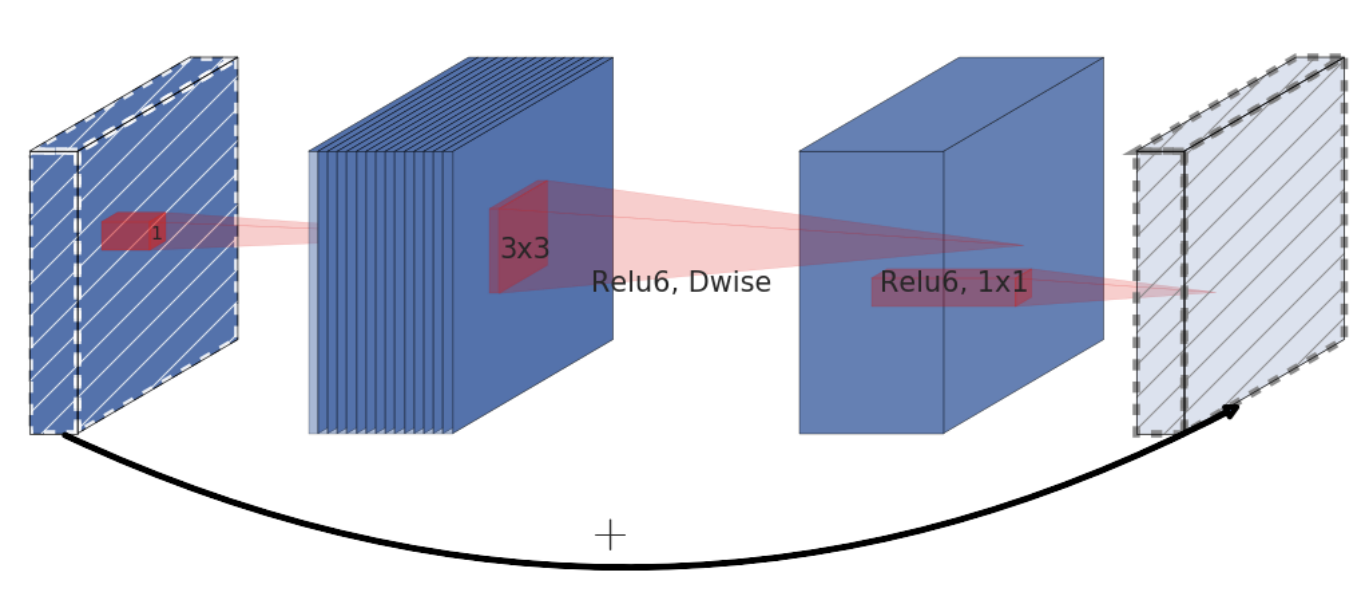
\includegraphics[width=7cm]{images/mbconv.png}
    \end{center}
    \label{mbconv_fig}
    \caption{An MBConv block with a depth-wise convolution applied to the middle layer, split into the 2 steps. The layers with the crosses do not have a non-linearity applied to them. Taken from \cite{sandler_howard_zhu_zhmoginov_chen_2018}}
\end{figure}

\subsection{Results}

The architecture search technique described above was able to achieve state-of-the-art results in a few different categories. On CIFAR-10 it got 2.08\% test error compared to 2.13\% which was achieved by AmoebaNet-B. It is a marginal improvement, but uses only 5.7 million parameters while the other network uses 34.9 million. On ImageNet evaluated on a GPU they also achieve state-of-the-art accuracy, getting 75.1\% while the previous is 72.0\%. When testing ImageNet on a mobile platform they achieve state-of-the-art accuracy when evaluation must be under 80ms getting theirs to run in 78ms and be 74.6\% accurate. Without using their latency regularization, the architecture search finds one with 158ms of latency on the Pixel 1, so it is definitely necessary to explicitly train for it. Their search cost is also much lower than the other methods. It takes 200 GPU hours to search for their architecture while the next best is 40,000 GPU hours.\\

\section{What we have learned in class}
Both the papers heavily use Gradient Descent to find an Optimal Neural Network Architecture. As discussed in class, Gradient Descent is an optimization algorithm that is used to minimize some function by iteratively moving in the direction of steepest descent as defined by the negative of the gradient. Gradient Descent is most commonly used to optimize the weights in a Neural Network. 
Using, Gradient Descent in both the proposed solutions although gave extremely efficient results during the experiments, but we cannot always guarantee to arrive at the Global Minima or attain an optimal result.


The PROXYLESS NAS paper uses latency for learning specialized network architectures on target hardware, it models network latency as a continuous function and optimizes it as regularization loss. Regularization is most commonly used to solve the overfitting problem. It  reduces the flexibility of the model by introducing a normalization function to our Loss function.

\bibliographystyle{ieeetr}
\bibliography{sources}
 
\end{document}